\begin{tehtavasivu}

\begin{tehtava}
	Osoita induktiolla, että luku $n^2+n$ on jaollinen luvulla $2$, kun $n$ on luonnollinen luku.
\end{tehtava}

\begin{tehtava}
	Osoita induktiolla, että luku $n^3+2n$ on jaollinen luvulla $3$, kun $n$ on luonnollinen luku.
\end{tehtava}

\begin{tehtava}
	Osoita induktiolla, että $2^n > n$, kun $n$ on luonnollinen luku.
\end{tehtava}

\begin{tehtava}
	Osoita induktiolla, että $n^2 > 2n + 1$, kun $n$ on kokonaisluku ja $n \ge 3$.
\end{tehtava}

\begin{tehtava}
	Osoita induktiolla, että luku $7^n + 5$ on jaollinen luvulla $6$, kun $n$ on positiivinen kokonaisluku.
\end{tehtava}

\begin{tehtava}
	Osoita induktiolla, että luku $10^n - 3^n$ on jaollinen luvulla $7$, kun $n$ on positiivinen kokonaisluku.
\end{tehtava}

\begin{tehtava}
	Osoita induktiolla, että luku $7^n - 6n + 8$ on jaollinen luvulla $9$, kun $n$ on positiivinen kokonaisluku.
\end{tehtava}

\begin{tehtava}
	Osoita induktiolla, että $n! > n^2$, kun $n$ on kokonaisluku ja $n \ge 4$. Merkintä $n!$ tarkoittaa luvun $n$ \termi{kertoma}{kertomaa}. Se on tulo $n! = n \cdot (n-1) \cdot (n-2) \cdot \ldots \cdot 3 \cdot 2 \cdot 1$.
\end{tehtava}

\begin{tehtava}
	Olkoot $n$ positiivinen kokonaisluku ja $r$ reaaliluku, jolle pätee $r \neq 1$. Osoita induktiolla, että 
	\[
	1 + r + r^2 + r^3 + \ldots + r^{n-1} = \frac{1-r^n}{1-r}.
	\]
\end{tehtava}

\begin{tehtava}
	Olkoon $n$ positiivinen kokonaisluku. Osoita induktiolla, että 
	\[
	1 \cdot 1! + 2 \cdot 2! + 3 \cdot 3! + \ldots + n \cdot n! = (n + 1)! - 1.
	\]
\end{tehtava}

\begin{tehtava}
	Osoita induktiolla, että 
	\[
	\sum_{m=1}^n m^2= \frac{n(n+1)(2n+1)}{6}, \textrm{ kun } n=1, 2, \ldots.
	\]
\end{tehtava}

\begin{tehtava}
	Osoita induktiolla, että $n$-alkioisessa joukossa on
	\[
	\frac{n(n-1)}{2}
	\]
	kahden alkion osajoukkoa, kun $n \ge 2$.
\end{tehtava}

\begin{tehtava}
	Todista kappaleessa 5.2 esiteltyjen kongruenssin laskusääntöjä koskevan lauseen kohta 4: Olkoot $a, b \in \zz$ ja $k, n \in \zz_+$ sekä $a \equiv b\ (\mod k)$. Tällöin $a^n \equiv b^n\ (\mod k)$.
\end{tehtava}

\begin{tehtava}
	Tarkastellaan kuviojonoa, joka muodostuu säännöllisen kuusikulmion muotoisista pistejoukoista. Jonon neljä ensimmäistä kuviota ovat seuraavat:

	\begin{center}
	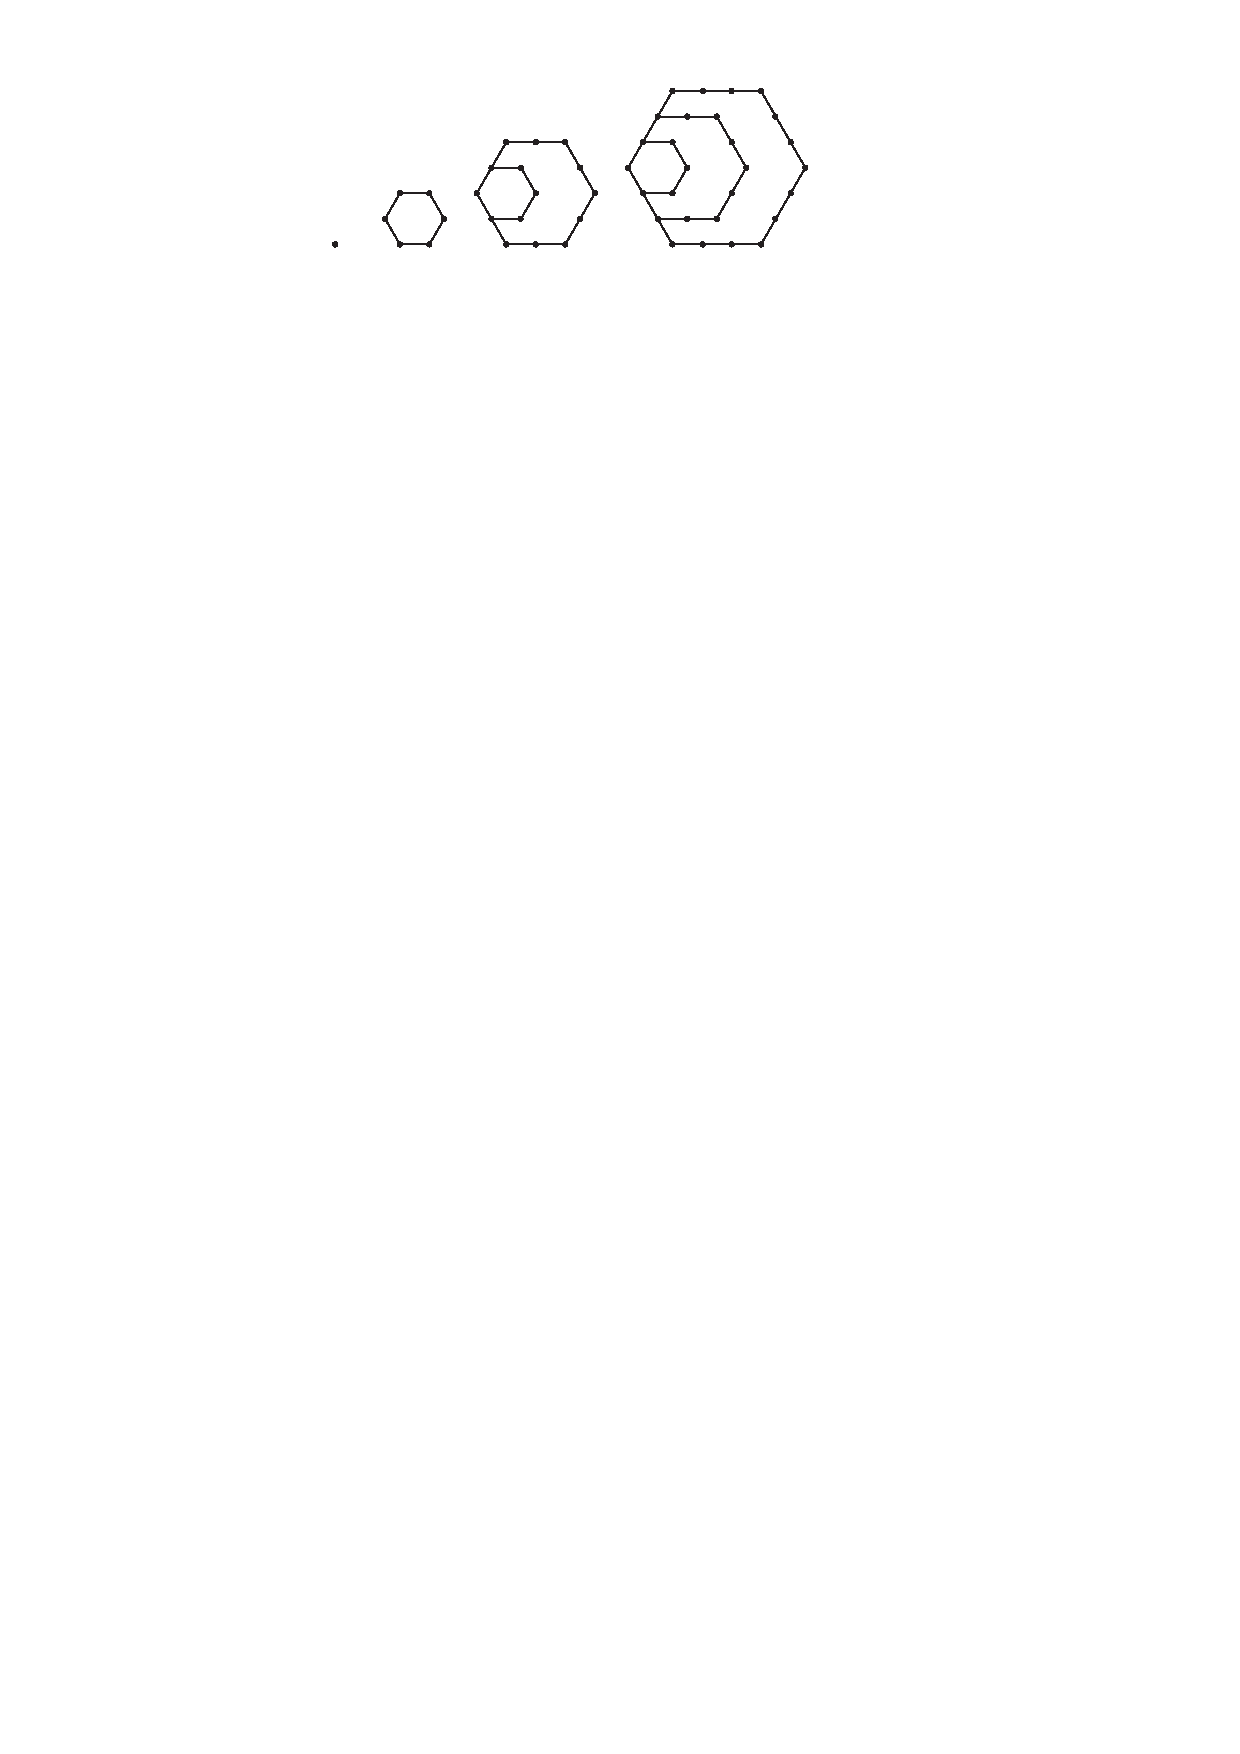
\includegraphics[width=10cm]{pictures/Kappale5_4_kuusikulm_v2}
	\end{center}


	\alakohdat{
	§ Laske, kuinka monta pistettä on kuviojonon kussakin neljässä ensimmäisessä kuviossa.
	§ Muodosta kaava, jolla voidaan laskea, kuinka monta pistettä on $n$. kuviossa. Tarpeen vaatiessa voit hyödyntää laskimesi polynomisovitustoimintoja.
	§ Todista kaava induktiolla.
	}
	
	\begin{vastaus}
	\alakohdat{
	§ 1, 6, 15, 28
	§ $2n^2 - n$
	}
	\end{vastaus}
\end{tehtava}

\end{tehtavasivu}

% -----


\begin{kotitehtavasivu}

\begin{tehtava}
	Osoita induktiolla, että $n$ jakopisteellä jana voidaan jakaa enintään $n + 1$ janaksi.

	\begin{center}
	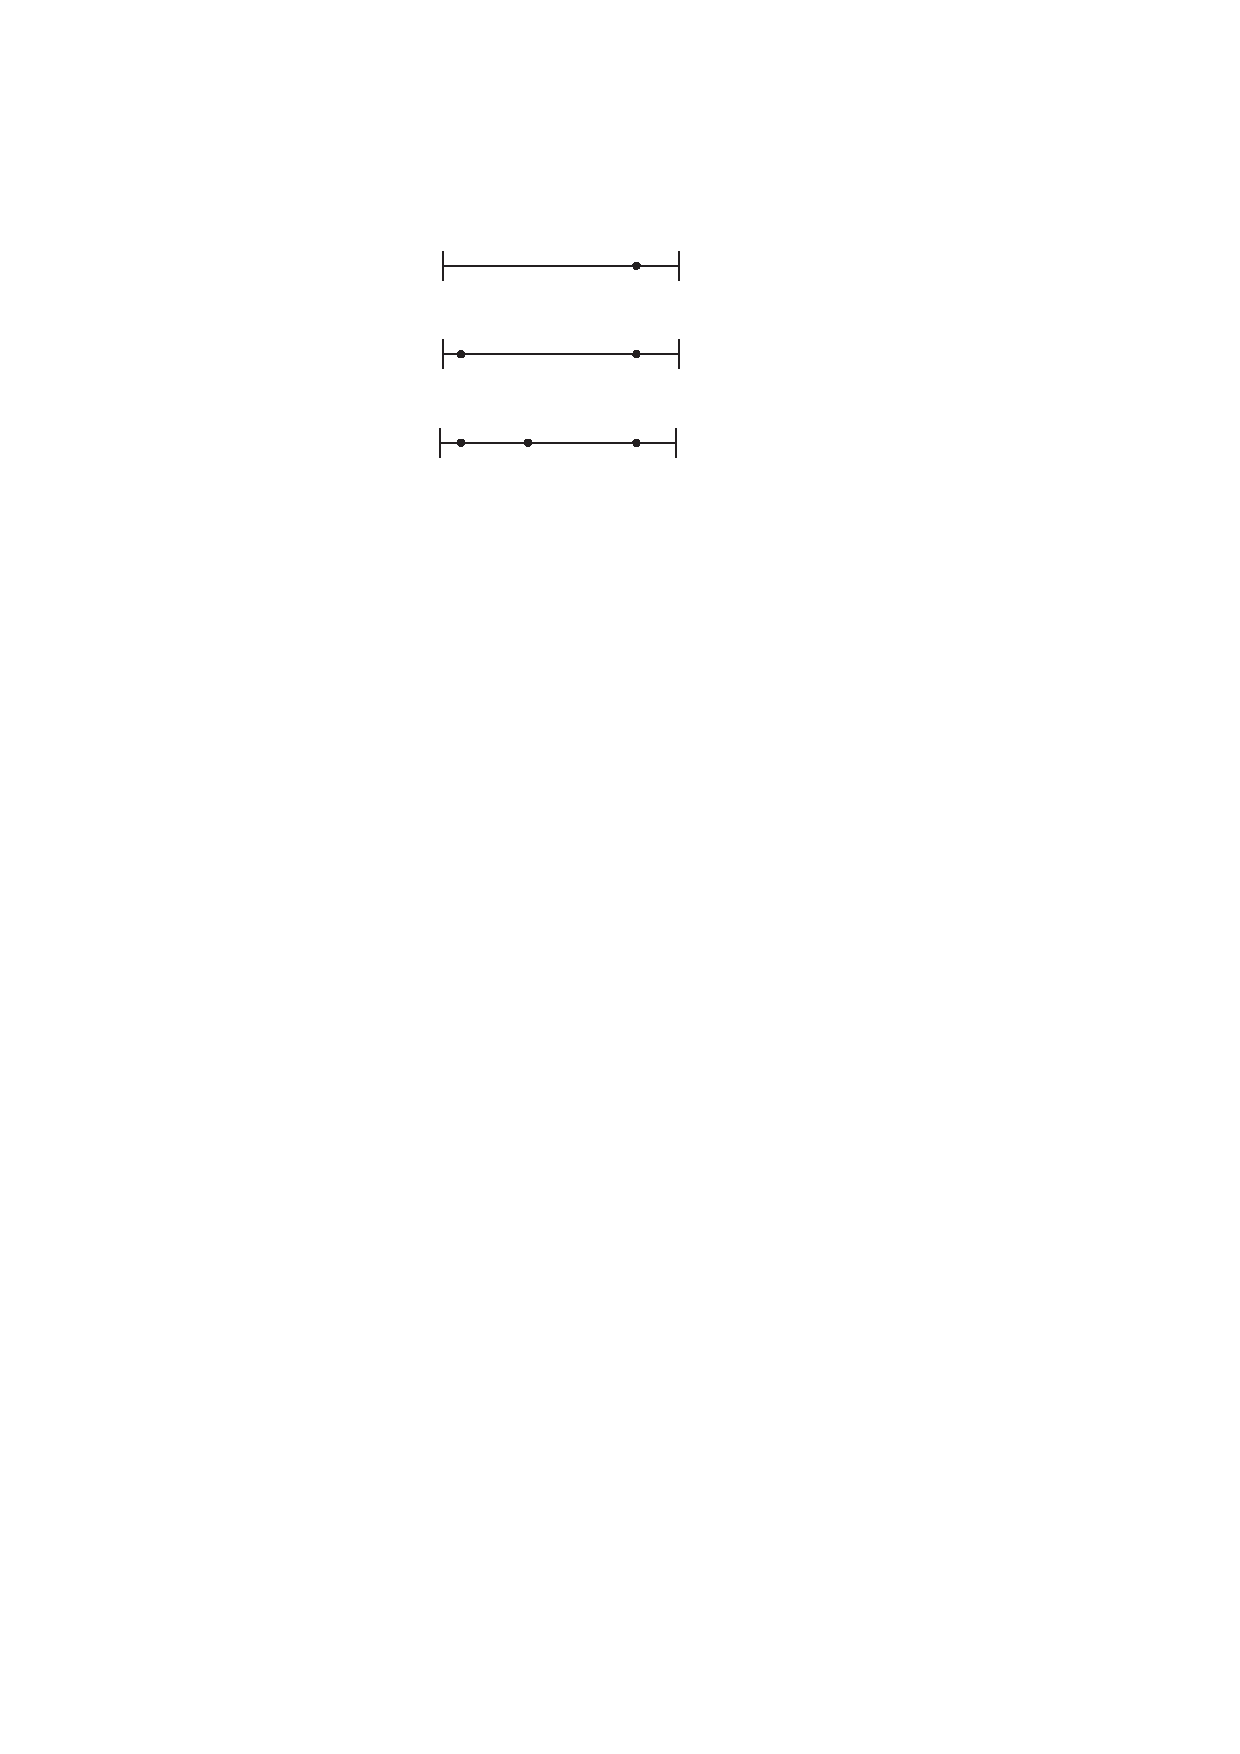
\includegraphics[width=6cm]{pictures/Kappale5_4_janat_v2}
	\end{center}
\end{tehtava}

\begin{tehtava}
	Osoita induktiolla, että luku $n^3 + 5n$ on jaollinen luvulla $6$, kun $n$ on luonnollinen luku.
\end{tehtava}

\begin{tehtava}
	Osoita, että $3^n > 2n$, kun $n$ on positiivinen kokonaisluku.
\end{tehtava}

\begin{tehtava}
	Osoita induktiolla, että $3^n < n!$, kun $n$ on kokonaisluku ja $n\ge 7$.
\end{tehtava}

\begin{tehtava}
	Osoita induktiolla, että luku $6^n - 1$ on jaollinen luvulla $5$, kun $n$ on positiivinen kokonaisluku.
\end{tehtava}

\begin{tehtava}
	Osoita induktiolla, että luku $8^n - 5^n$ on jaollinen luvulla $3$, kun $n$ on positiivinen kokonaisluku.
\end{tehtava}

\begin{tehtava}
	Osoita induktiolla, että luku $27^{2n} + 3 \cdot 13^{n}$ on jaollinen luvulla $4$, kun $n$ on positiivinen kokonaisluku.
\end{tehtava}

\begin{tehtava}
	Osoita induktiolla, että
	\[
	\sum_{m=1}^n m^3= \frac{n^2(n+1)^2}{4}, \textrm{ kun } n=1, 2, \ldots.
	\]
\end{tehtava}

\begin{tehtava}
	Osoita induktiolla, että $(1 + 2 + 3 +\ldots + n)^2 = 1^3 + 2^3 + 3^3 + \ldots + n^3$, kun $n$ on positiivinen kokonaisluku.
\end{tehtava}

\begin{tehtava}
	Tasoon piirretään $n$ suoraa ($n\ge 2$). Osoita, että suorilla voi olla korkeintaan $n(n - 1)/2$ leikkauspistettä.
\end{tehtava}

\begin{tehtava}
	Tarkastele seuraavia luvun $2$ peräkkäisistä potensseista muodostuvia summia:
	\[
	\begin{array}{rcl}
	1 &=& 1\\
	1 + 2 &=& 3\\
	1 + 2 + 4 &=& 7\\
	1 + 2 + 4 + 8 &=& 15\\
	1 + 2 + 4 + 8 + 16 &=& 31\\
	1 + 2 + 4 + 8 + 16 + 32 &=& 63\\
	1 + 2 + 4 + 8 + 16 + 32 + 64 &=& 127.
	\end{array}
	\]
	Muodosta kaava, jolla voidaan laskea summa $2^0 + 2^1 + 2^2 + \ldots + 2^n$, missä $n$ on luonnollinen luku. Todista kaava induktiolla.
	
	\begin{vastaus}
		$2^{n+1}-1$
	\end{vastaus}
\end{tehtava}

\begin{tehtava}
	Olkoot $n$ luonnollinen luku ja $x$ reaaliluku, jolle pätee $x > -1$. Osoita, että $(1 + x)^n \ge 1 + nx$. Kyseessä on niin sanottu \termi{Bernoullin epäyhtälö}{Bernoullin epäyhtälö}.
\end{tehtava}

\begin{tehtava}
	Olkoon $n$ positiivinen kokonaisluku. Todista, että
	\[
	\frac{1}{2}\le\frac{1}{n+1}+\frac{1}{n+2}+\ldots +\frac{1}{n+n} <1.
	\]
	[YO syksy 1971 tehtävä 7]
\end{tehtava}

\begin{tehtava}
	Osoita, että kaikilla positiivisilla kokonaisluvuilla $n$ on
	\[
	1^2+3^2+5^2+\ldots+(2n-1)^2 = \frac{n(4n^2-1)}{3}. 
	\]
	[YO kevät 1998 8b]
\end{tehtava}

\begin{tehtava}
	Tarkastellaan ruudukoista muodostuvaa kuviojonoa, jonka neljä ensimmäistä kuviota ovat seuraavat:

	\begin{center}
	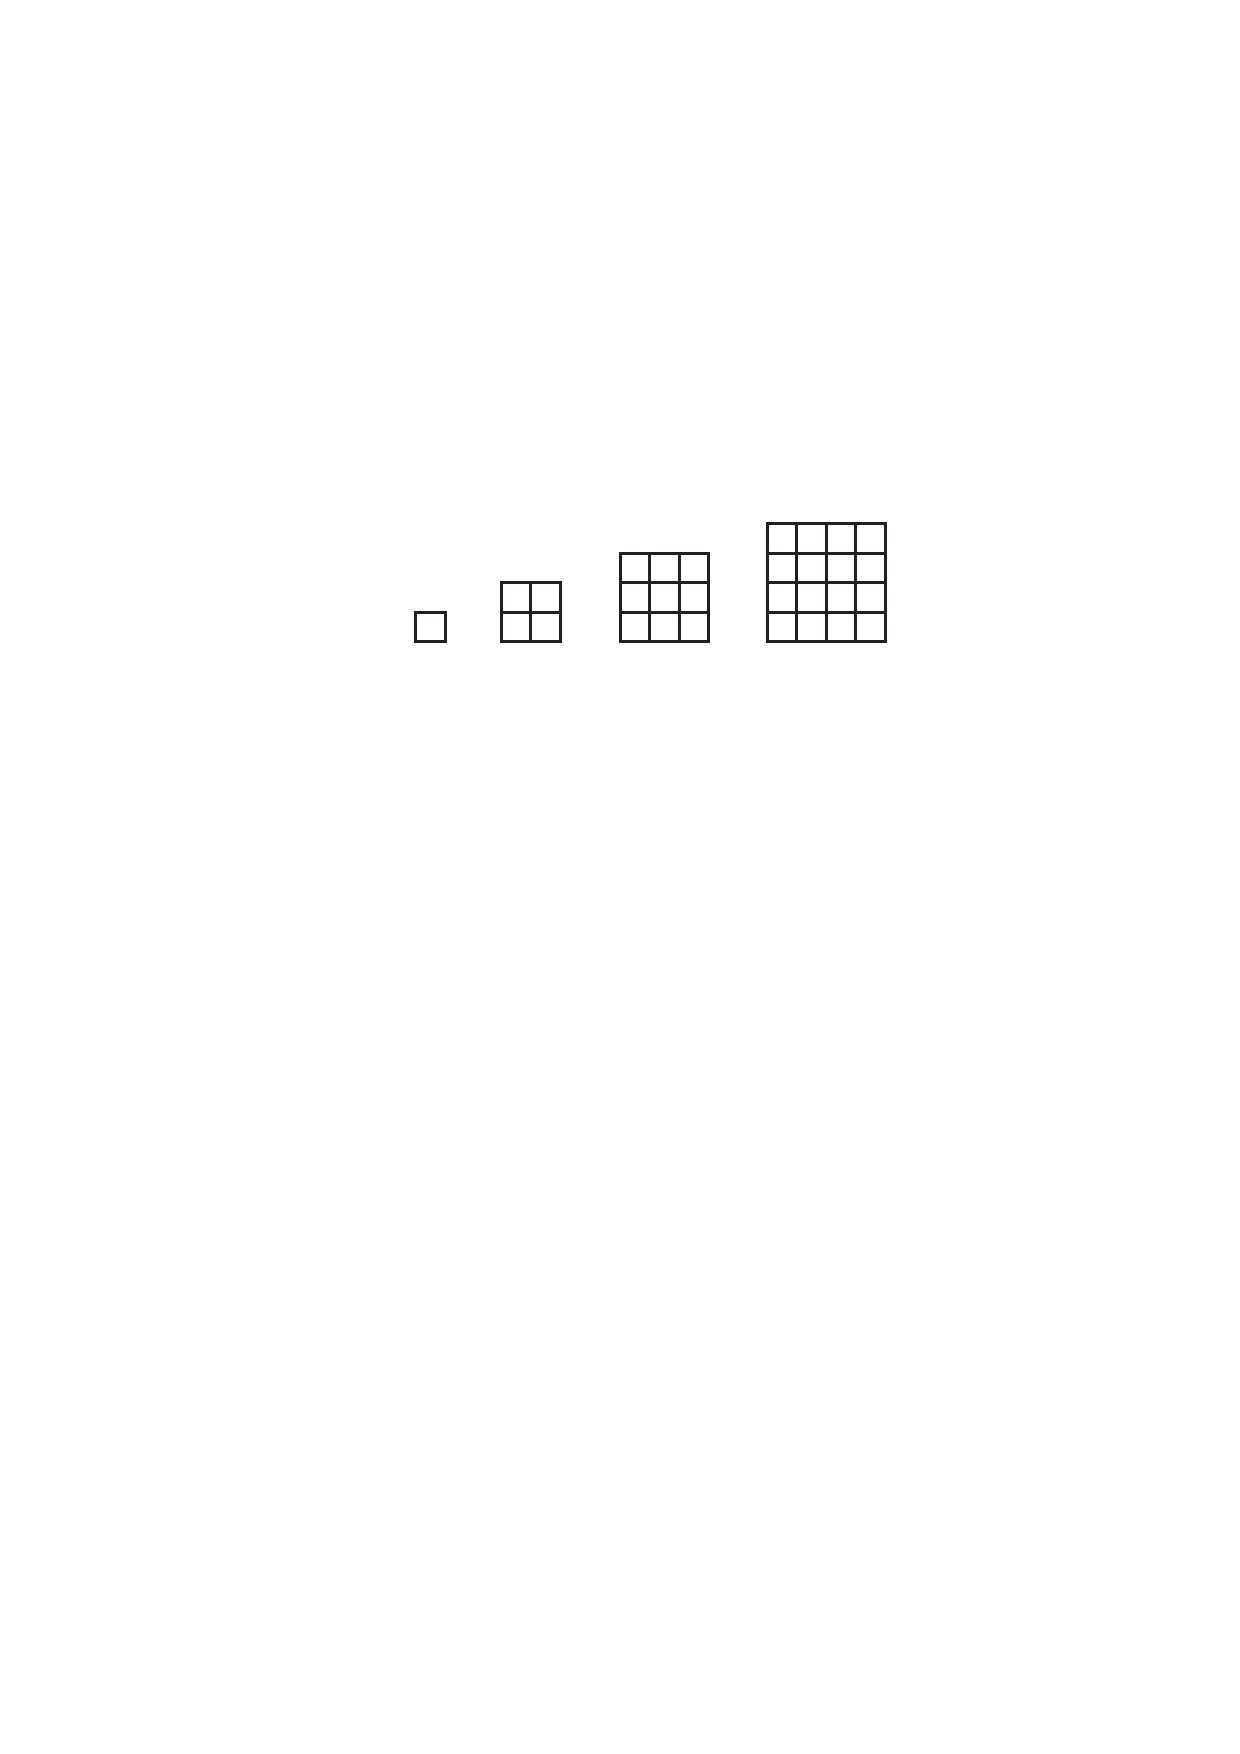
\includegraphics[width=10cm]{pictures/Kappale5_4_ruudukko_v2}
	\end{center}

	\alakohdat{
	§ Kuvioihin muodostuu erikokoisia neliöitä. Laske, kuinka monta neliötä kaikkiaan on kuviojonon kussakin neljässä ensimmäisessä ruudukossa.
	§ Muodosta kaava, jolla voidaan laskea, kuinka monta neliötä on $n$. ruudukossa. Tarpeen vaatiessa voit hyödyntää laskimesi polynomisovitustoimintoja.
	§ Todista kaava induktiolla.
	}
	
	\begin{vastaus}
	\alakohdat{
	§ $1$, $5$, $14$, $30$
	§ $\frac{2n^3 + 3n^2 + n}{6}$
	}
	\end{vastaus}
\end{tehtava}

\begin{tehtava}
	Eräs keino, jolla voi tarkastaa onko yhteenlasku oikein suoritettu, perustuu seuraavaan lauselmaan:

	Jos useampien kokonaislukujen summa ja samoin näiden lukujen numerosummien summa jaetaan yhdeksällä, niin tulevat jäännökset yhtä suuriksi. Todista tämä lauselma.
	[YO 1895 tehtävä 2]
\end{tehtava}

\end{kotitehtavasivu}
